% Local-only guide; commands executed on the acceptance date unless stated otherwise.
\chapter{INSTALLATION AND USER GUIDE}\label{app:installation}

\section{Installation Requirements}
\subsection{Hardware Requirements}
The application runs on one local computer and needs no GPU. Every figure in this appendix was
recorded on \nAppHost{}. With the ridge model, the API and the worker together peaked at
\nAppPeakMemory{}~MB during the largest recorded job. The optional LoRA-D model raises the API to
about \nAppApiMemLora{}~MiB and needs roughly 40~s of processor time per tile on this machine. Offline
research training has separate requirements, given in Section~\ref{sec:research-local-guide}.

\subsection{Software Requirements}
Two installations are supported. The container installation needs only Docker Engine with Compose
version~2 and the repository's local data directory, which the reference loader reads read-only. The
host installation needs Python~3.12 with a virtual environment, Node~24 to build the interface, and
optionally a PostgreSQL~16 container; exact package versions are pinned by the requirement files and
the interface lockfile. Either installation is checked in a recent Chromium, Firefox or WebKit
browser. The research runner additionally uses its own packages and MMseqs2; these are not required
for serving predictions.

\section{Local System Execution}
There is one local web application. Public hosting, VPS, domain and TLS deployment are outside the
required workflow, and every listener binds to the loopback address.

\subsection{Container Installation}
From \nolinkurl{system/app}, \texttt{make docker-env} writes a local configuration file with a
random database password. \texttt{docker compose up -d -{}-build db} starts PostgreSQL~16,
\texttt{make docker-etl} loads the reference data and the model weights after checking their
hashes, and \texttt{make docker-up} starts the API, the worker and the web server. The interface is
then at \nolinkurl{http://127.0.0.1:8080}; it is the only published port. The API migrates the
database on start, so the \nAppMigrations{} migrations need not be invoked separately. With the full
ClinVar subset, the reference load took \nAppEtlSeconds{}~s.
\texttt{make docker-dev} starts the same services with hot reload for development, and
\texttt{make docker-test} and \texttt{make docker-e2e} run the test suites against them.

Setting \texttt{WITH\_LORA=1} in the configuration builds the backend image with PyTorch, and the
loader registers LoRA-D when its exported bundle is present. The ridge model stays the default unless
the configuration names LoRA-D as the default model.

\subsection{Host Installation}
From \nolinkurl{system/app}, \texttt{make venv} creates the backend environment; in
\nolinkurl{frontend}, \texttt{npm ci} and \texttt{npm run build} build the interface.
\texttt{make etl SCOPE=in-tiles} prepares a SQLite reference database. \texttt{make dev-api}
and \texttt{make dev-worker} then start the API on \nolinkurl{http://127.0.0.1:8000} and the job
worker in two terminals, or one process runs both when the worker is embedded. A clean installation
of this kind into an empty directory, including reference preparation, took
\nAppInstallSeconds{}~s. To use PostgreSQL instead, \texttt{make pg-up} starts a PostgreSQL~16
container and the loader and the API are pointed at it through the database URL.

The health endpoint should report that the model is loaded and the database reachable; if the model
weights do not match their registered hash, the service reports a degraded state and refuses to score
rather than serving an unverified artefact. For backup, copy the database and the workspace file
directory together, because an uploaded import is referenced from the database by a generated path.
Reference data can always be rebuilt by running the loader again; saved analyses and imported
datasets cannot.

\section{User Guide}
The screens below were captured from the running application with reference data and the ridge
model; the four screens shown in Chapter~\ref{chap:design} are not repeated. A typical session runs
as follows.

\textbf{1. Create or open a project.} The project list and a project's history are shown in
Figure~\ref{fig:guide-projects}. Deleting a project first shows what depends on it.

\textbf{2. Choose the input.} A single peptide gives a quick preview that is saved only on request;
a peptide batch or a whole protein runs as a durable job. For a protein, search by gene symbol or
accession, then review the summary before submitting: length, number of windows, uncovered residues
and the domain outcome (Figure~\ref{fig:guide-input}, top). For a single tile, choose it on the tile
map, where each window shows its domain status (Figure~\ref{fig:guide-input}, bottom).

\textbf{3. Read the result.} The effect matrix and its footprint track
(Figure~\ref{fig:app-matrix}) open below the domain banner and warnings. Use the ranking, the
shortlist and the top-$k$ panel to choose substitutions; scroll to the footprint track to see where in
the window the signal lies (Figure~\ref{fig:guide-saved}, top). A whole-protein job reports progress
per window (Figure~\ref{fig:app-job}) and keeps each window's result separate.

\textbf{4. Save and reopen.} A saved analysis is an immutable snapshot; reopening it shows the result
with the model, gate and annotations of the day it was saved (Figure~\ref{fig:guide-saved}, bottom).
Rerunning creates a new entry.

\textbf{5. Read the context.} The ClinVar tab lists the missense variants of the tile with their
classification and the diagnostic disclaimer (Figure~\ref{fig:guide-context}, top). The model page
(Figure~\ref{fig:app-model}) and the sources page (Figure~\ref{fig:guide-context}, bottom) state
what a score means, which data it rests on and under which licences.

\textbf{6. Import and compare.} Import a CSV or TSV file with its assay, endpoint, units and source
(Figure~\ref{fig:guide-import}, top), read the validation report, and commit it explicitly
(Figure~\ref{fig:guide-import}, bottom). A committed dataset can then be compared with a saved
analysis (Figure~\ref{fig:app-comparison}). Imported values never retrain the model, and a comparison
is not independent validation.

\textbf{7. Export.} Each result, job and comparison exports as CSV or JSON with its model, hashes,
sources, versions and the development-evidence label.

\begin{figure}[htbp]
  \centering
  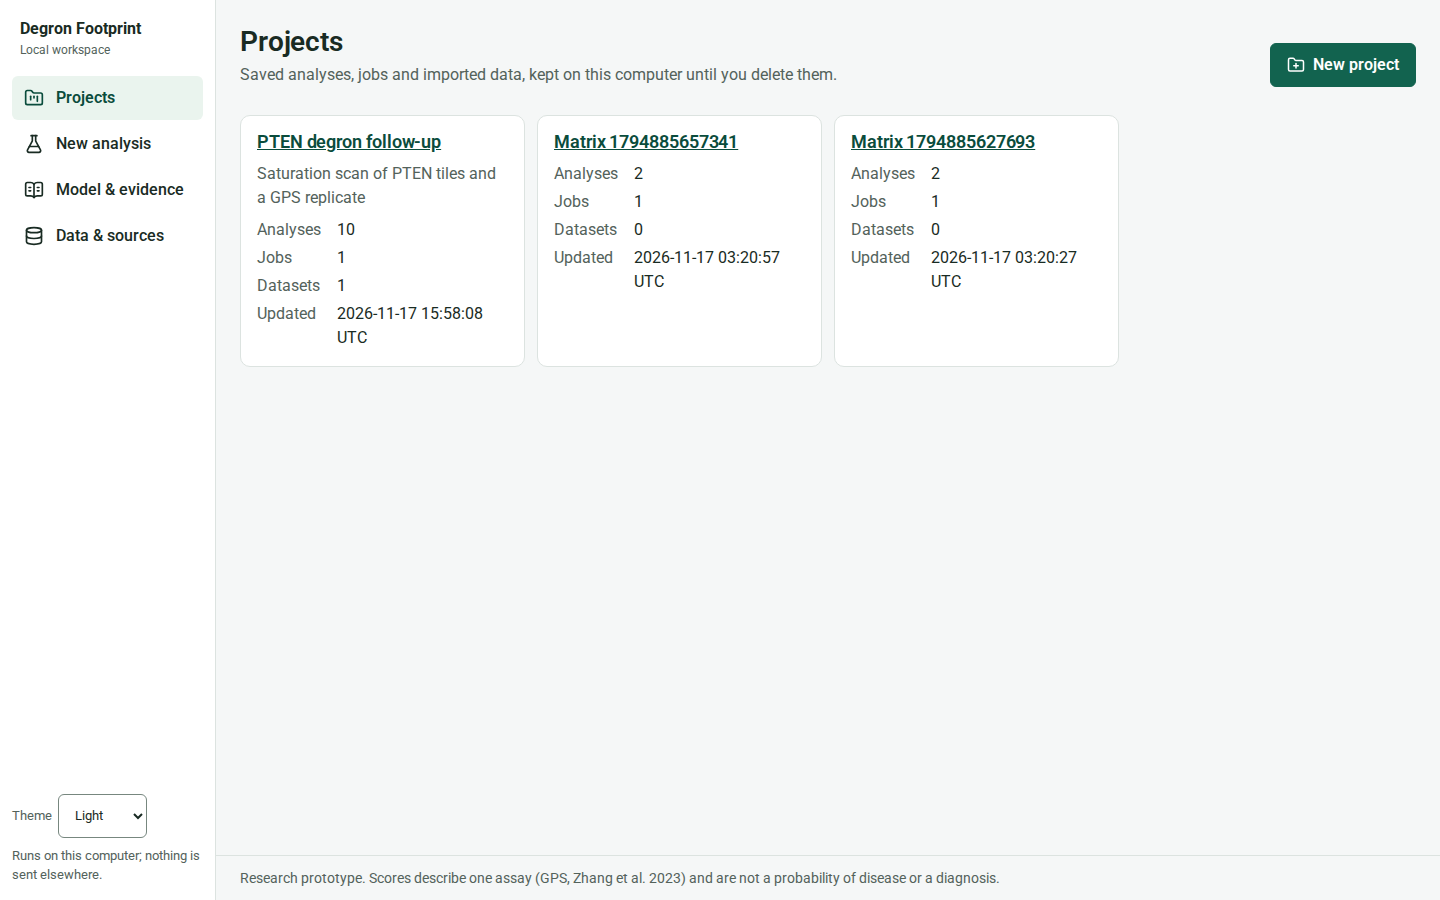
\includegraphics[width=0.74\textwidth]{assets/screenshots/01-projects.png}\par\medskip
  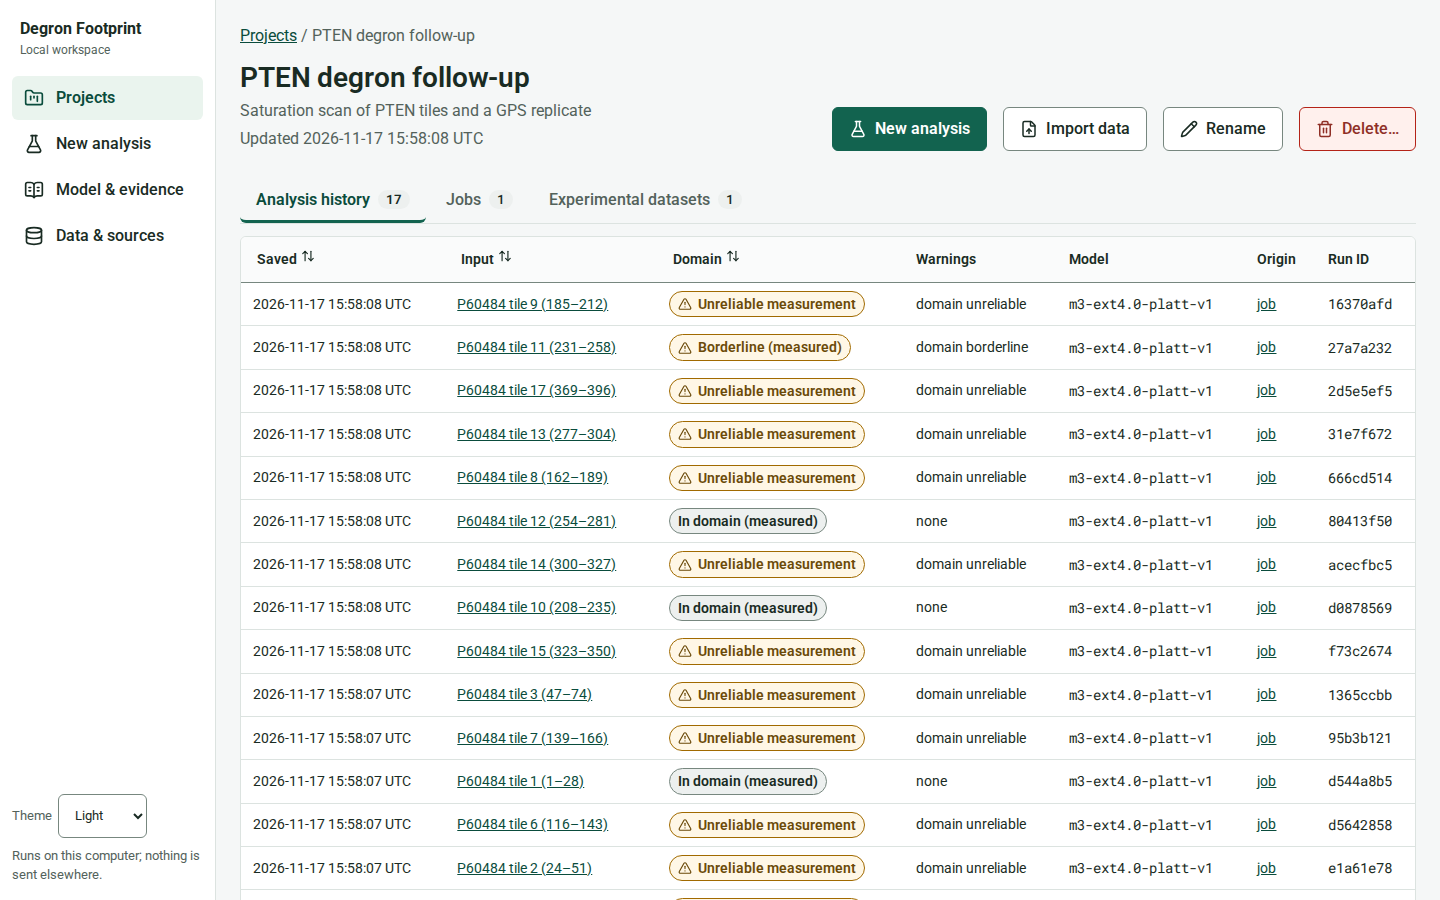
\includegraphics[width=0.74\textwidth]{assets/screenshots/02-project-history.png}
  \caption[Projects and analysis history]{Projects and analysis history (UC-10). Top: the project list with the number of analyses, jobs
  and datasets in each. Bottom: the history of one project, where every saved analysis keeps its
  domain status, warnings and the model that produced it.}
  \label{fig:guide-projects}
\end{figure}

\begin{figure}[htbp]
  \centering
  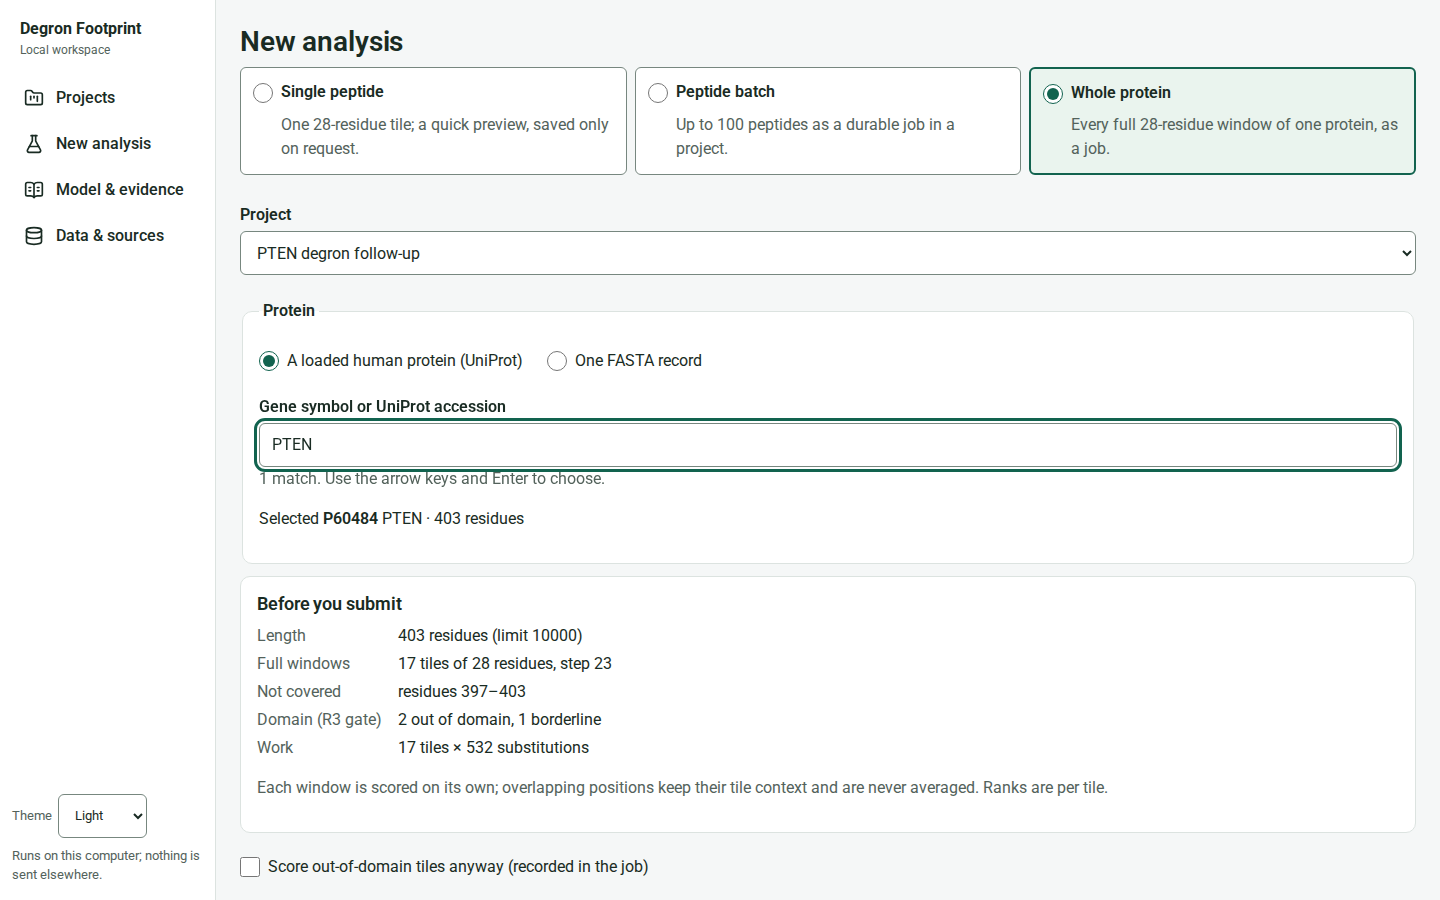
\includegraphics[width=0.74\textwidth]{assets/screenshots/03-new-analysis-protein.png}\par\medskip
  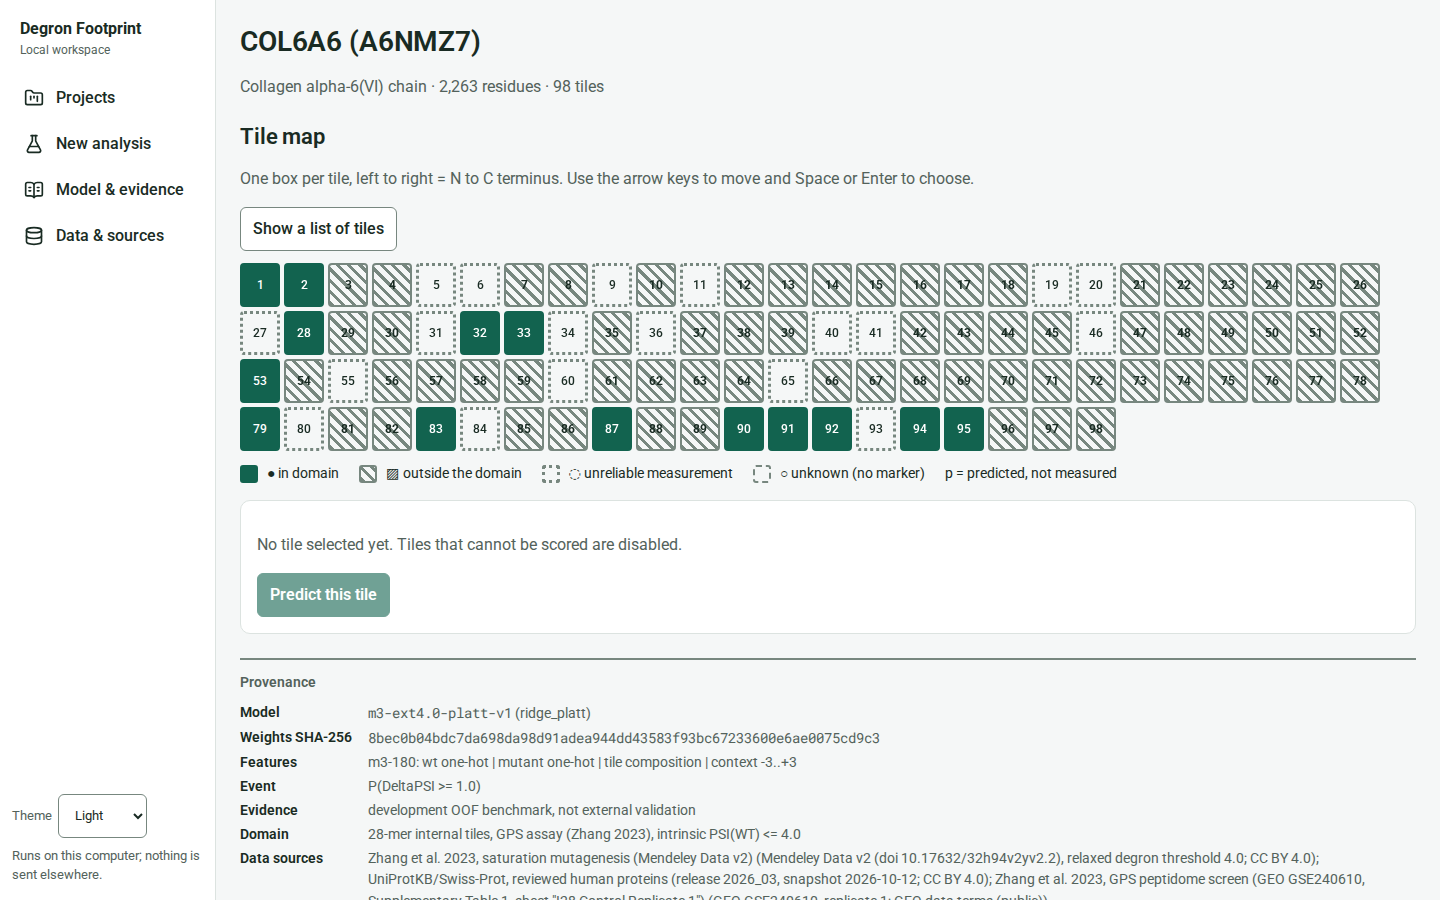
\includegraphics[width=0.74\textwidth]{assets/screenshots/04-tile-picker.png}
  \caption[Choosing the input]{Choosing the input (UC-04, UC-08). Top: a whole-protein job with the summary shown before
  submission, including the uncovered terminal residues and the domain outcome. Bottom: the tile map
  of a protein with the domain status of every window; tiles that cannot be scored are disabled.}
  \label{fig:guide-input}
\end{figure}

\begin{figure}[htbp]
  \centering
  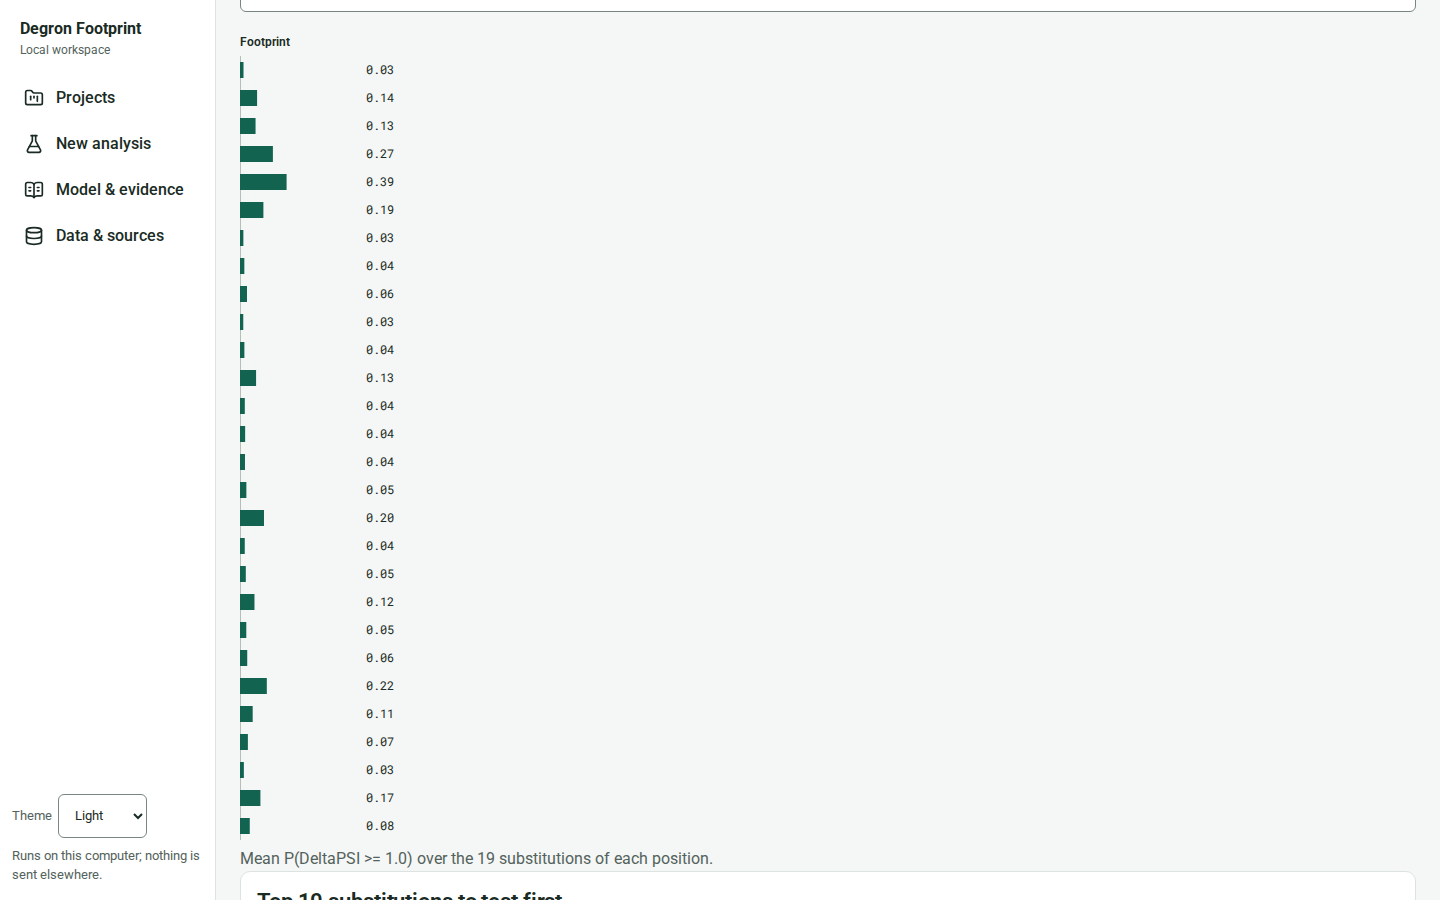
\includegraphics[width=0.74\textwidth]{assets/screenshots/05b-footprint-track.png}\par\medskip
  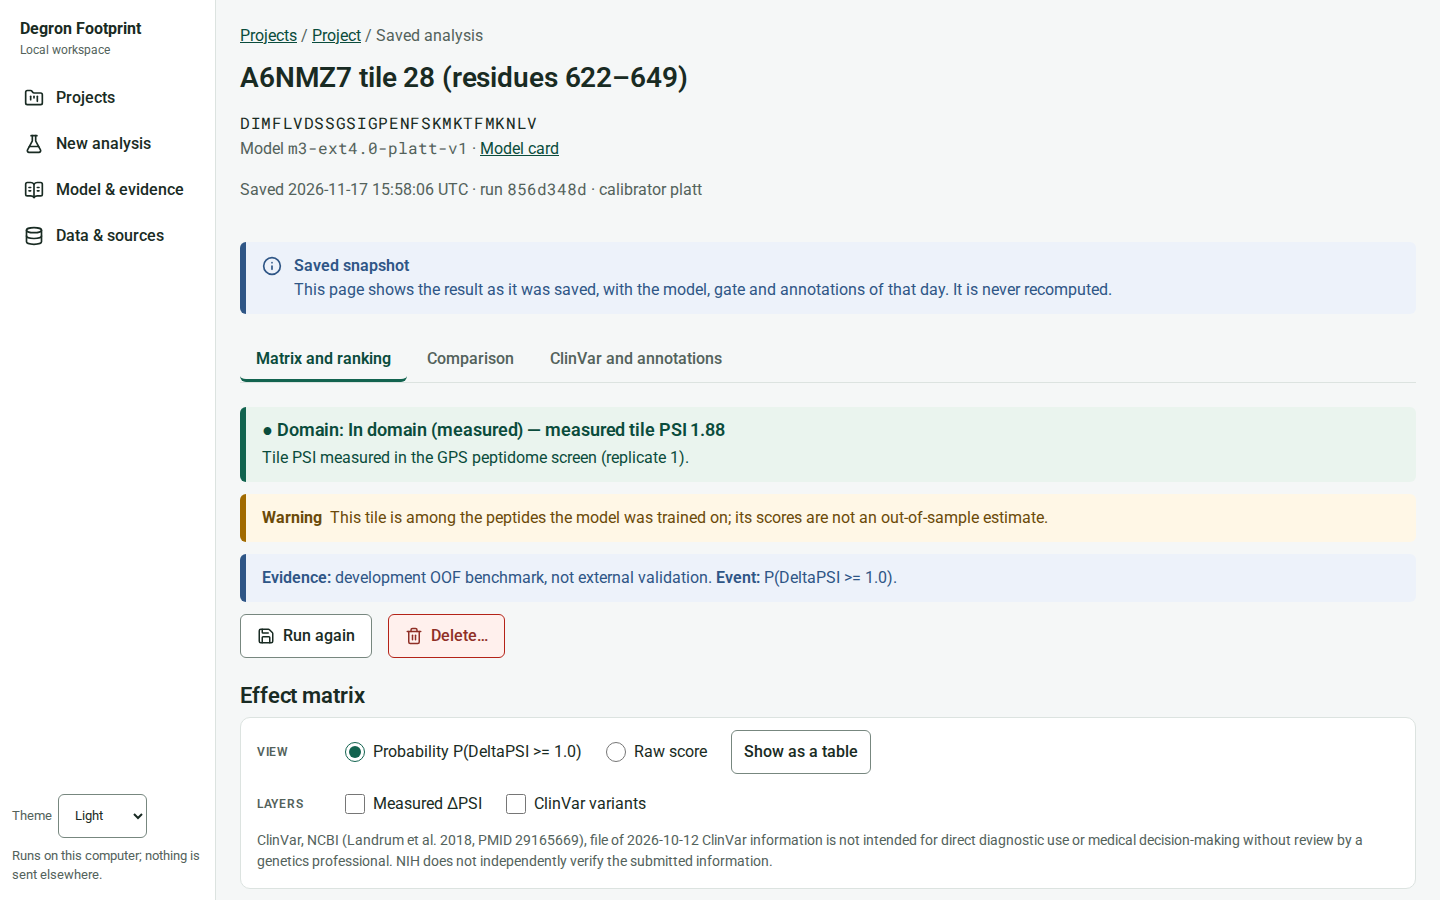
\includegraphics[width=0.74\textwidth]{assets/screenshots/07-saved-analysis.png}
  \caption[Footprint track and a saved snapshot]{Footprint track and a saved snapshot (UC-01, UC-10). Top: the mean probability over the
  nineteen substitutions of each position. Bottom: a reopened analysis, which is shown as it was
  saved and is never recomputed.}
  \label{fig:guide-saved}
\end{figure}

\begin{figure}[htbp]
  \centering
  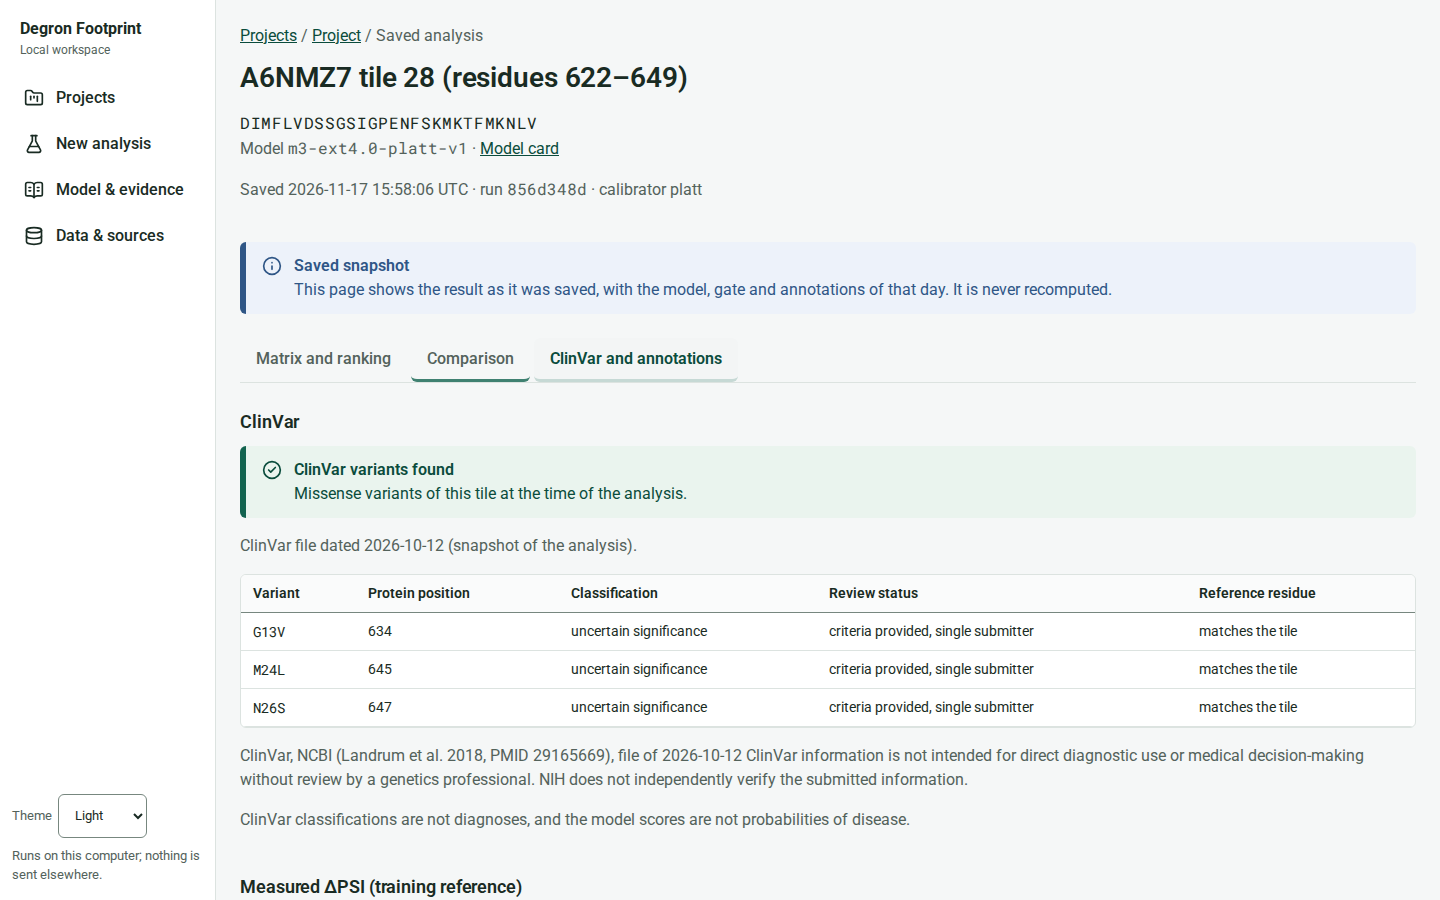
\includegraphics[width=0.74\textwidth]{assets/screenshots/09-annotations.png}\par\medskip
  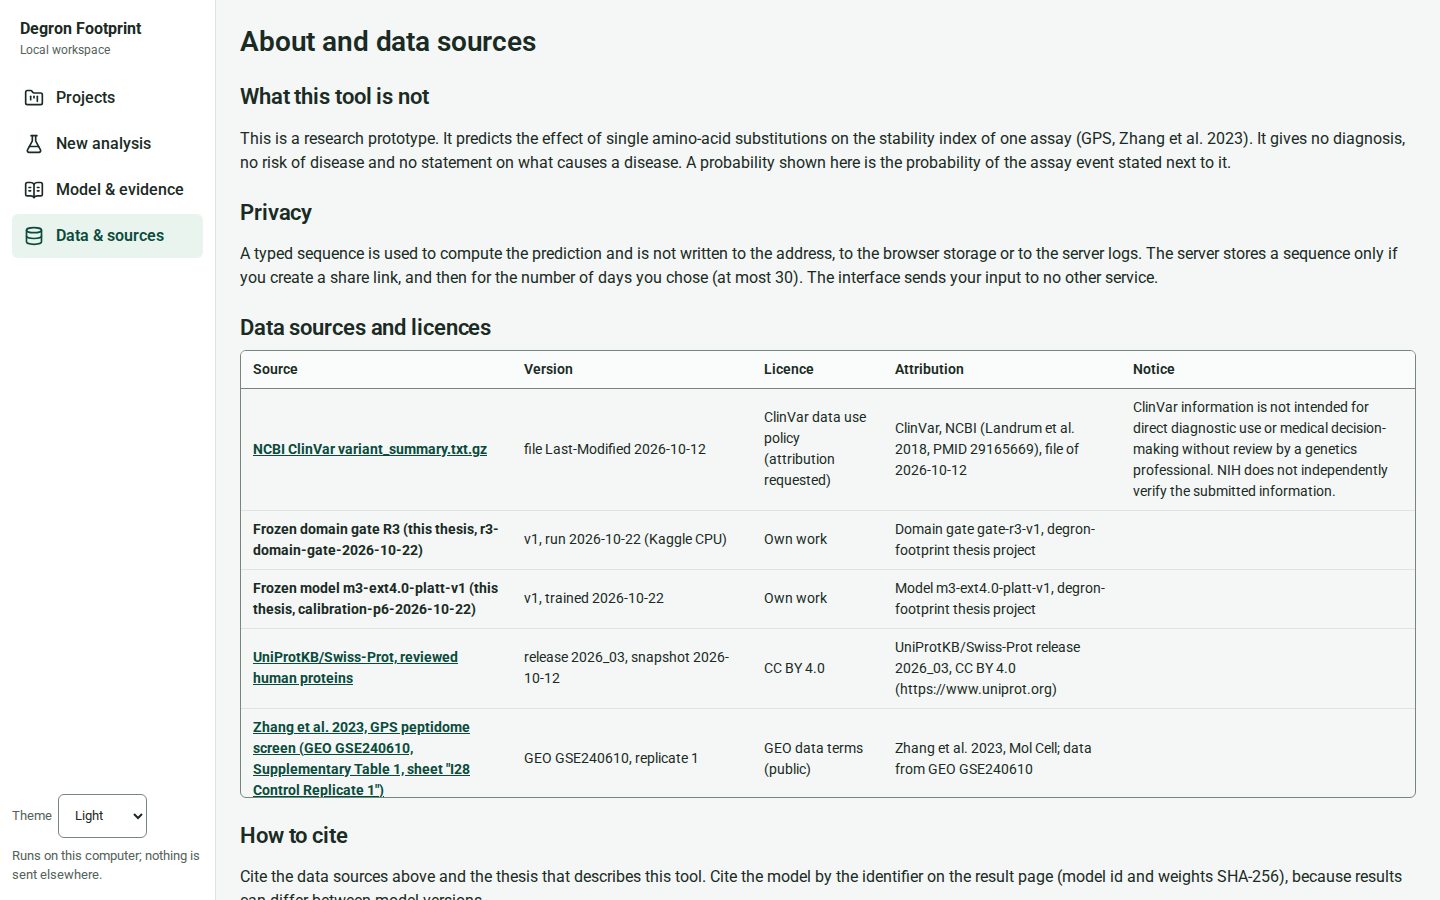
\includegraphics[width=0.74\textwidth]{assets/screenshots/13-sources.png}
  \caption[ClinVar annotations and data sources]{ClinVar annotations and data sources (UC-06, UC-07). Top: ClinVar missense variants of a
  tile with attribution and the statement that the information is not for diagnostic use. Bottom: the
  sources page with versions and licences. The privacy note on that page still mentions a share link
  from the retired requirement FR-20; the share link is not a feature of this release.}
  \label{fig:guide-context}
\end{figure}

\section{Offline Research Campaign Workflow}\label{sec:research-local-guide}
The research supervisor is separate from the application's API and job worker. It uses the pinned
full-PSI data bundle, pretrained-weight caches and a CUDA environment. From PowerShell at the
repository root, \nolinkurl{./status-local.cmd} inspects the campaign. To execute or resume permitted
work, \texttt{./run-local.cmd -{}-hours 2} starts a visible session. Request a safe pause using
\nolinkurl{./pause-local.cmd} or Ctrl+C in that session. Training commits recovery checkpoints
approximately every 120 seconds; an abrupt window close can lose work since the last commit.
These are the operational commands of the campaign; the report itself does not rerun them.

The graph first checks the runtime/data identity and imported reference outputs, then verifies
tokenizer alignment and extracts frozen features for each cached checkpoint. It runs the family ridge
grid and matched frozen/LoRA tuning, collects OOF predictions, fits CV calibrators, evaluates the
locked W5-D transfer recipe and writes the final report. Complete jobs are skipped when resuming
the same compatible campaign; previous source output must remain available for inherited artifacts.
Changing code, data, protocol or relevant runtime properties can create a new identity and must not
be bypassed by editing a manifest or copying arbitrary checkpoints.

On 6 November the runnable graph had 633 completed jobs and two pending input-dependent
extensions; the later refit of Section~\ref{sec:transfer-refit} ran as a separate campaign with its own
identity. A session that reports zero executed jobs and then ends has no eligible compute left;
restarting it alone does not provide the missing reviewed external or structure inputs. No further
training is needed to reproduce the present analysis from the saved artifacts. Cached model/data
work can be read offline; acquiring new sources or absent model/dependency files is a preparation
step that may require connectivity.

For evidence regeneration, enter the research campaign directory and run
\texttt{python analyze-local-output.py}. This reads saved OOF artifacts, verifies provenance and
recomputes analysis without loading trained checkpoint objects. From the repository root,
\texttt{python} \nolinkurl{research/output-review-2026-11-06/audit.py}
rechecks selected source hashes and exports the full evidence inventory. The report-asset generator
then rebuilds tables and scientific figures from the exported JSON. Regeneration is an analysis task;
it does not promote a candidate into the application.

\subsection{Campaign Recovery and Execution Environment}\label{sec:campaign-methods}
The execution unit is a dependency-tracked job with pinned code, data, model revision, protocol and
runtime identity. The Kaggle run supplies the reference experiments; the Windows successor expands
the pLM family and completes a matched frozen--LoRA comparison. These runs use the same development
population, but different software and GPU environments. They are retained as separate estimates.

Figure~\ref{fig:campaign-lineage} shows how interrupted work is recovered. Completed outputs can be
inherited only after compatibility and checksum checks. The tokenizer-repair successor reuses 456
completed jobs from the earlier local campaign; it does not count those jobs twice. Paused training
uses committed checkpoints, including optimiser and random-state information. A timer-failure run
that produced no scientific OOF predictions is superseded. A final report job denotes completion of
the runnable graph; missing reviewed external and structure inputs remain explicit pending states.

\begin{figure}[htbp]
  \centering
  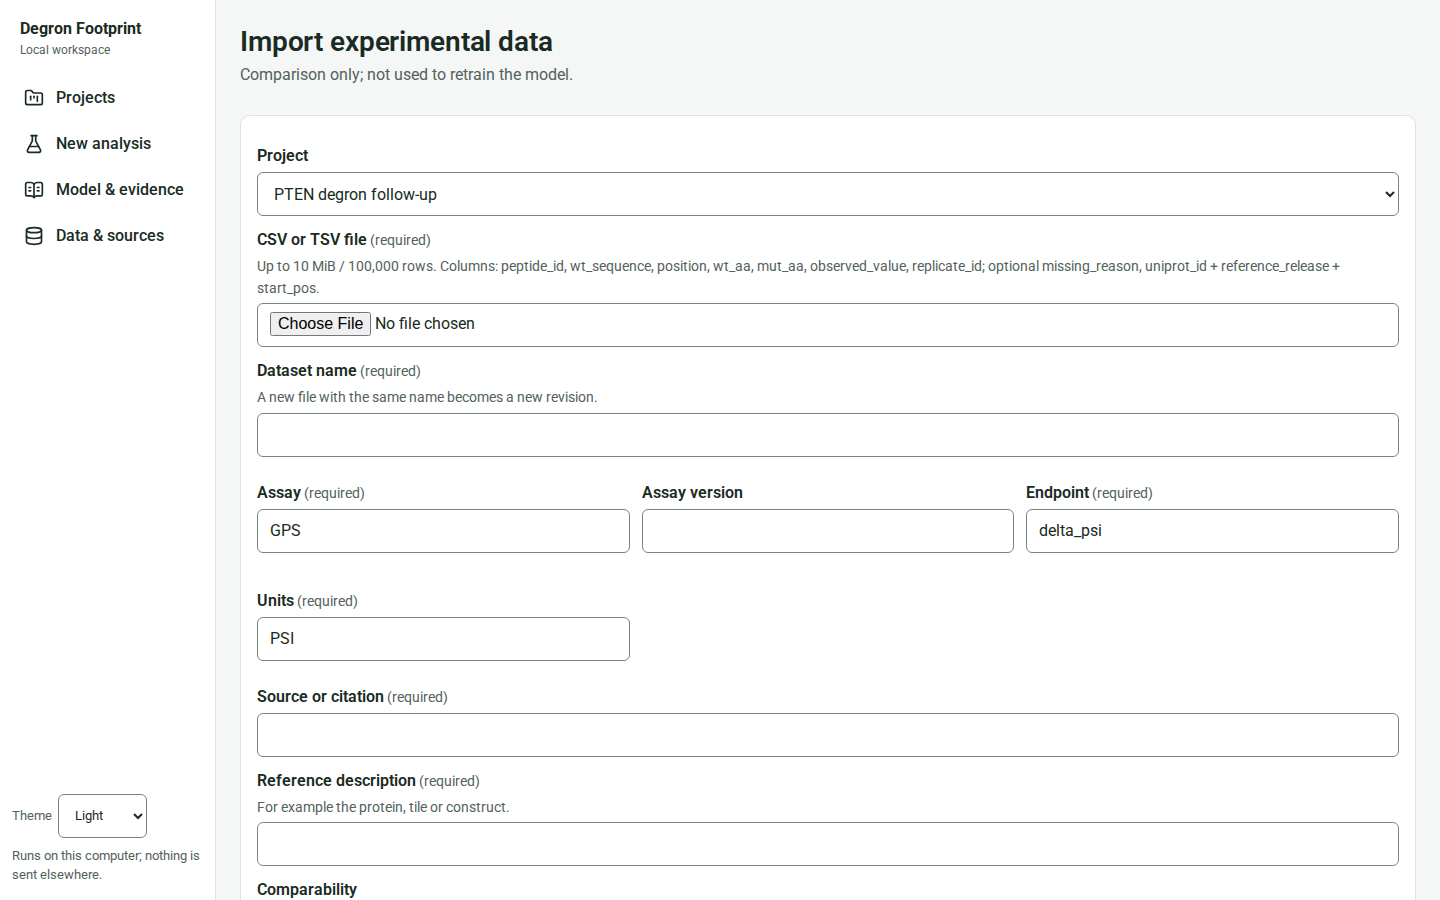
\includegraphics[width=0.74\textwidth]{assets/screenshots/10-import.png}\par\medskip
  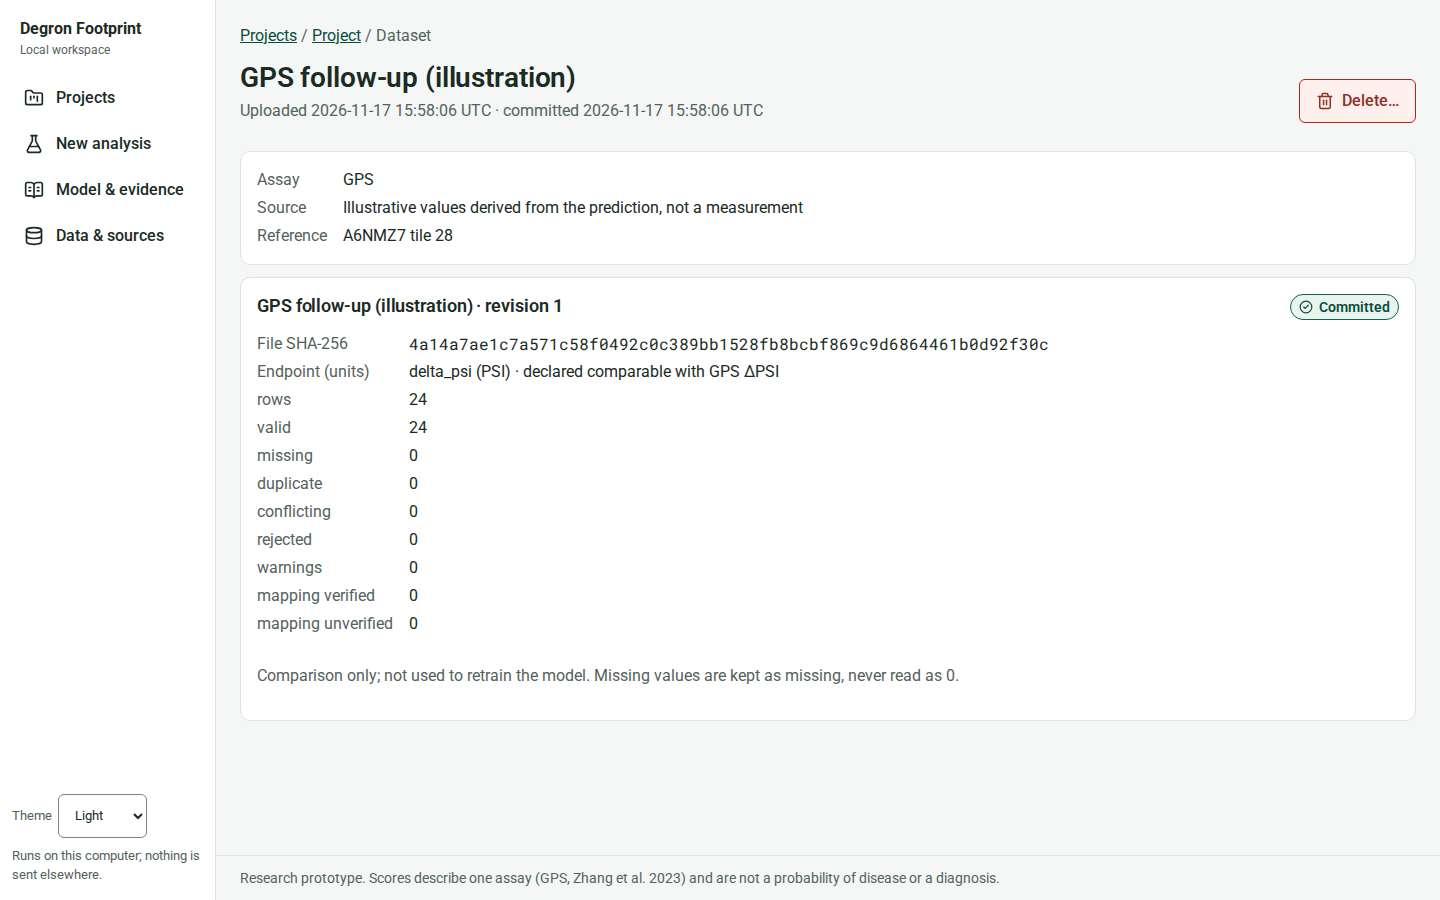
\includegraphics[width=0.74\textwidth]{assets/screenshots/11-dataset.png}
  \caption[Importing experimental data]{Importing experimental data (UC-09). Top: the import form, which requires assay,
  endpoint, units and source. Bottom: a committed dataset with its validation counts. The values in
  this illustration were derived from a prediction, not measured, and the dataset says so.}
  \label{fig:guide-import}
\end{figure}

The local environment is Python 3.11.9, PyTorch 2.13.0 with CUDA 13.0, Transformers 5.17.0 and
an RTX 5060 Laptop GPU with approximately 8~GiB memory. Model/tokenizer weights are cached and
revision-pinned. ProtT5 initially reached a misleading tokenizer fallback requesting \texttt{tiktoken};
installing the missing Protobuf dependency restored its intended tokenizer. Ankh uses the original
fast tokenizer with residue-level input and an FP32 encoder because FP16 hidden states were
non-finite. ProtT5 uses FP16 encoding; stored family features use FP16. These execution choices are
recorded parts of the recipes, so this is not a controlled comparison of pretraining alone.

\begin{figure}[htbp]
  \centering
  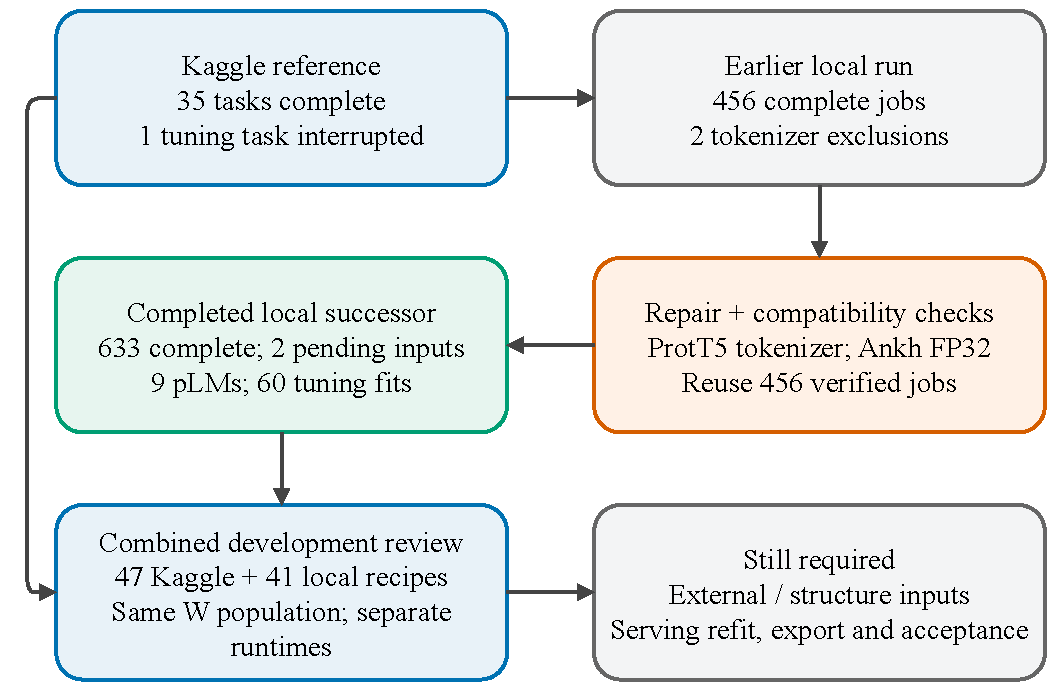
\includegraphics[width=\textwidth]{assets/diagrams/campaign-2026-11-06/campaign-lineage.pdf}
  \caption[Campaign lineage and evidence roles at completion on 6 November 2026]{Campaign lineage and evidence roles at completion on 6 November 2026.
  Inheritance preserves compatible work; the combined review does not create independent datasets.}
  \label{fig:campaign-lineage}
\end{figure}


